\documentclass[10pt,landscape]{article}
\usepackage{multicol}
\usepackage{calc}
\usepackage{ifthen}
\usepackage[landscape]{geometry}
\usepackage{graphicx}
\usepackage{amsmath, amssymb, amsthm}
\usepackage{latexsym, marvosym}
\usepackage{pifont}
\usepackage{lscape}
\usepackage{array}
\usepackage{booktabs}
\usepackage[bottom]{footmisc}
\usepackage{tikz}
\usetikzlibrary{shapes}
\usepackage{pdfpages}
\usepackage{wrapfig}
\usepackage{enumitem}
\setlist[description]{leftmargin=0pt}
\usepackage{xfrac}
\usepackage{xcolor}

% --- XELATEX ADJUSTMENT HERE ---
% Removed 'pdftex' driver option. XeLaTeX handles this automatically.
\usepackage[
            pdfauthor={Karim Luna},
            pdftitle={Control Cheatsheet},
            pdfsubject={A cheatsheet pdf based on my study and research},
            % hidelinks % Optional: hides those ugly red/green boxes around links
            ]{hyperref}
% -------------------------------

\usepackage[open, openlevel=2]{bookmark}
\usepackage{relsize}
\usepackage{rotating}
\usepackage{titlesec}


% Math & Logic Commands
\newcommand\independent{\protect\mathpalette{\protect\independenT}{\perp}}
\def\independenT#1#2{\mathrel{\setbox0\hbox{$#1#2$}%
\copy0\kern-\wd0\mkern4mu\box0}} 

% CHANGE LATER KARIM
% \newcommand{\Bin}{\textrm{Bin}}
% \newcommand{\Beta}{\textrm{Beta}}
% \newcommand{\Gam}{\textrm{Gamma}}
% \newcommand{\Expo}{\textrm{Expo}}
% \newcommand{\Pois}{\textrm{Pois}}
% \newcommand{\Unif}{\textrm{Unif}}
% \newcommand{\Geom}{\textrm{Geom}}
% \newcommand{\NBin}{\textrm{NBin}}
% \newcommand{\HGeom}{\textrm{HGeom}}
% \newcommand{\Mult}{\textrm{Mult}}
\newcommand{\real}{\textrm{Re}}

% Style
\definecolor{wine-red}{rgb}{0.6, 0, 0}
\geometry{top=.4in,left=.2in,right=.2in,bottom=.4in}

\pagestyle{empty}
\setcounter{secnumdepth}{0}

\setlength{\parindent}{0pt}
\setlength{\parskip}{0pt plus 0.5ex}

% Section Formatting
\titleformat{\section}
{\color{red}\normalfont\sffamily\large\bfseries} % Added \sffamily
{\thesection}{1em}{}
\titlespacing*{\section}{0pt}{1.2ex}{0.6ex}

\titleformat{\subsection}
{\color{wine-red}\normalfont\sffamily\normalsize\bfseries} % Added \sffamily
{\thesubsection}{1em}{}
\titlespacing*{\subsection}{0pt}{1ex}{0.5ex}

\begin{document}

\raggedright
\footnotesize
\begin{multicols*}{3}

% multicol parameters
\setlength{\premulticols}{1pt}
\setlength{\postmulticols}{1pt}
\setlength{\multicolsep}{1pt}
\setlength{\columnsep}{2pt}

%%%%%%%%%%%%%%%%%%%%%%%%%%%%%%%%%%%%
%%% TITLE
%%%%%%%%%%%%%%%%%%%%%%%%%%%%%%%%%%%%

\begin{center}
    {\color{black} \Large{ \sffamily\textbf{Control Systems}}} \\
\end{center}

%%%%%%%%%%%%%%%%%%%%%%%%%%%%%%%%%%%%
%%% ATTRIBUTIONS
%%%%%%%%%%%%%%%%%%%%%%%%%%%%%%%%%%%%

\scriptsize
Created by Karim Luna \hfill Last Updated \today

\vspace{2pt}
\hrule
\vspace{4pt}

%%%%%%%%%%%%%%%%%%%%%%%%%%%%%%%%%%%%
%%% BEGIN CHEATSHEET
%%%%%%%%%%%%%%%%%%%%%%%%%%%%%%%%%%%%

% \section{Definitions}


\section{Laplace Transform} \smallskip \hrule height 2pt \smallskip

    \subsection{Definition} 

    \begin{center}
        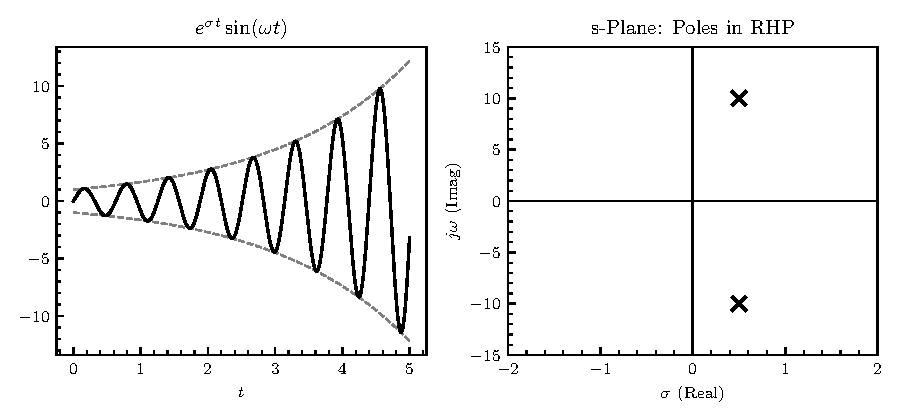
\includegraphics[width=3in]{figures/laplace.pdf}
    \end{center}

    The Laplace transform is a generalized Fourier transform used to simplify differential equations, either transforming PDEs into ODEs or converting ODEs into algebraic expressions. It is specifically designed to handle functions that grow exponentially at infinity. By definition, we have:
    \begin{align*}
        \mathcal{L} \{f(t)\} = F(s) = \int_0^\infty f(t)e^{-st},dt
    \end{align*}
    In control theory, this transform is used to convert the time-domain equations of a dynamic system into a s-domain transfer function, making it easy to see if the natural response is unbounded (i.e., identifying poles with positive real parts).
    \newline

    Let $f(t)=e^{\sigma t}sin(\omega t), t\geq0$, be a modulated signal, where $\sigma$ is the growth rate and $\omega$ is the angular frequency.
    Taking the Laplace transform yields
    \begin{align*}
        F(s)=\frac{\omega}{(s-\sigma)^2+\omega^2},
    \end{align*}
    by setting the denominator to zero
    \begin{align*}
        \boxed{s = \sigma \pm j\omega = 0.5 \pm j10},
    \end{align*}
    because $\real(s)=\sigma>0$ these poles lie in the Right-Half Plane (RHP), representing a unstable, exponentially growing oscillation of the time-domain signal. 
    
    \subsection{Essential pairs}

    \renewcommand{\arraystretch}{1.3}
    \begin{center}
    \begin{tabular}{cc}
    \hline
    $f(t), t>0 $                & F(s)        \\
        \hline
        $\delta (t)$            & 1           \\
        u(t) (unit step)        & $\frac{1}{s}$ \\ 
        t (unit ramp)           & $\frac{1}{s^2}$ \\ 
        $t^n$                   & $\frac{n!}{s^{n+1}}$ \\
        $e^{at}$                & $\frac{1}{s+a}$ \\
        $\sin (\omega t)$       & $\frac{\omega}{s^2+\omega^2}$ \\
        $\cos (\omega t)$       & $\frac{s}{s^2+\omega^2}$ \\
        $e^{at}\sin (\omega t)$ & $\frac{\omega}{(s+a)^2+\omega^2}$ \\
        $e^{at}\cos (\omega t)$ & $\frac{s+a}{(s+a)^2+\omega^2}$ \\

    \end{tabular}
    \end{center}

    \subsection{Properties}
    These equations represent the differentiation and integration properties of the Laplace transform,
    \begin{align*}
        &\mathcal{L}\{\dot{f}\} =sF(s)-f(0), \\
        &\mathcal{L}\{\ddot{f}\}=s^2F(s)-sf(0)-\dot{f}(0), \\
        &\mathcal{L}\left\{\int_0^t f d\tau \right\}=\frac{F(s)}{s}, \\
    \end{align*}
    But in general we almost always assume zero initial conditions so $f(0)=0$.
    \newline

    The final value theorem is valid if and only if all poles of $sF(s)$ are in the Left-Half Plane (LHP),
    \begin{align*}
        \lim_{t\rightarrow\infty}f(t)=\lim_{s\rightarrow0}sF(s),
    \end{align*}    
    And is a tool used to verify a steady-state output or final value as time approaches infinity.


    \subsection{From frequency domain to time domain}
    Let $F(s)$ be a rational Laplace transform from which we wish to find the time response $f(t)$. The most direct approach is to expand $F(s)$ into a sum of simpler terms. 

    For distinct real poles, the expansion is given by:
    \begin{align*}
        F(s)=\frac{N(s)}{(s+a)(s+b)}=\frac{A}{s+a}+\frac{B}{s+b},\\[1mm]
        A=\lim_{s\rightarrow -a}(s+a)F(s),\quad B=\lim_{s\rightarrow -b}(s+b)F(s).
    \end{align*}
    Finding $A$ and $B$ and then applying the inverse Laplace transform is straightforward.
    \newline

    However, if $F(s)$ contains a second-order repeated pole at $s = -a$, the function takes the form:
    \begin{align*}
        F(s) = \frac{N(s)}{(s+a)^2} &= \frac{A_1}{s+a} + \frac{A_2}{(s+a)^2}, \\[1mm]
        A_2 = \lim_{s\rightarrow -a}(s+a)^2 F(s), &\quad A_1 = \lim_{s\rightarrow -a}\frac{d}{ds}\left[(s+a)^2 F(s)\right].
    \end{align*}
    The derivative is required for $A_1$ to isolate the lower-power coefficient. The resulting inverse Laplace transform introduces a time-multiplied exponential mode:
    \begin{align*}
        \boxed{f(t) = A_1 e^{-at} + A_2 t e^{-at}, \quad t \ge 0}
    \end{align*}

\section{Transfer Functions and Block Algebra}\smallskip \hrule height 2pt \smallskip
    \subsection{Derivation}
    The input ($u$) and output ($y$) behavior of a linear time-invariant (LTI) system can be modeled by a linear differential equation of the form,
    \begin{align*}
        a_0\frac{d^ny}{dt^n}+a_1\frac{d^{n-1}y}{dt^{n-1}}+\cdots+a_ny=b_0\frac{d^mu}{dt^m}+b_1\frac{d^{m-1}u}{dt^m}+\cdots+b_mu,
    \end{align*}
    where $n\ge m$ and $a_k,b_k\in\mathbf{R}$. To derivate the transfer funciton G(s) we just have to write the governing ODE, apply Laplace term by term ($u\rightarrow U(s), y\rightarrow Y(s)$) and solve for $Y(s)/U(s)$. Thus,
    \begin{align*}
        G(s)=\frac{\mathcal{L}[\text{output}]}{\mathcal{L}[\text{input}]}\Bigg|_{\text{zero initial conditions}}
    \end{align*}


\end{multicols*} 
\end{document}